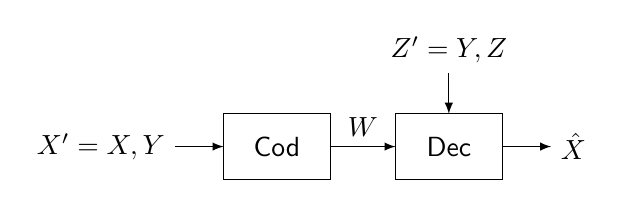
\begin{tikzpicture}[scale=0.52,>=latex]
    \tikzstyle{every node}=[font=\fontsize{10}{12}\sffamily]

    \draw[->] (0,0.8) node[left]{\(X'=X,Y\)} -- (1.2,0.8);

    \draw (1.2,0) rectangle (3.8,1.6)
    node[midway,align=center]{Cod};

    \draw[->] (3.8,0.8) -- (5.4,0.8)
    node[above,midway]{\(W\)};

    \draw (5.4,0) rectangle (8,1.6)
    node[midway,align=center]{Dec};

    \draw[->] (8,0.8) -- (9.2,0.8)
    node[right]{\(\hat{X}\)};

    \draw[<-] (6.7,1.6) -- (6.7,2.6)
    node[above]{\(Z'=Y,Z\)};
\end{tikzpicture}
